\documentclass[12pt, a4paper, onepage, english,singlespacing, parskip]{scrartcl}

%\documentclass[
%11pt, % The default document font size, options: 10pt, 11pt, 12pt
%oneside, % Two side (alternating margins) for binding by default, uncomment to switch to one side
%chapterinoneline,% Have the chapter title next to the number in one single line
%english, % ngerman for German
%singlespacing, % Single line spacing, alternatives: onehalfspacing or doublespacing
%draft, % Uncomment to enable draft mode (no pictures, no links, overfull hboxes indicated)
%nolistspacing, % If the document is onehalfspacing or doublespacing, uncomment this to set spacing in lists to single
%liststotoc, % Uncomment to add the list of figures/tables/etc to the table of contents
%toctotoc, % Uncomment to add the main table of contents to the table of contents
%parskip, % Uncomment to add space between paragraphs
%nohyperref, % Uncomment to not load the hyperref package
%headsepline, % Uncomment to get a line under the header
%]{scrartcl or scrreprt or scrbook} % The class file specifying the document structure

\usepackage{lmodern} 		% Diese beiden packages sorgen für echte 
\usepackage[T1]{fontenc}	% Umlaute.

\usepackage{amssymb, amsmath, color, graphicx, float, setspace, tipa}
\usepackage[utf8]{inputenc} 
\usepackage[english]{babel}
\usepackage[pdfpagelabels,pdfstartview = FitH,bookmarksopen = true,bookmarksnumbered = true,linkcolor = black,plainpages = false,hypertexnames = false,citecolor = black, breaklinks]{hyperref}
\usepackage{url}
\usepackage{picins} 		%Gleittext um Grafik. Befehl: parpic. Vorlage siehe unten
\usepackage{longtable} 		%Seitenübergreifende Tabelle. Vorlage siehe unten
\usepackage{caption}
\captionsetup{font=small,labelfont=bf, format=plain, justification=centering}
\allowdisplaybreaks % allows page breaks in align/equation environment

\usepackage{authblk} % titlepage stuff
\usepackage[titletoc, title]{appendix}

%--------------------------------------------
% NEUE BEFEHLE
%--------------------------------------------
% Gleich mit Dach obendrauf
%\newcommand{\entspricht}{\mathrel{\widehat{=}}}
% Atanh
%\newcommand {\arctanh}{\mathrm{arctanh}}
% Acotanh
%\newcommand{\arccot}{\mathrm{arccot }}
% Limes von etwas gegen null
%\newcommand{\limz}[1]{\lim\limits_{#1 \rightarrow 0}}
%Bold font in math
%\newcommand{\bm}{\boldmath}
%\newcommand{\dps}{\displaystyle}
% e noncursive in math mode
%\newcommand{\e}{\mbox{e}}
% partial diff operator
%\newcommand{\del}{\partial}
%--------------------------------------------
%--------------------------------------------
%---------OPTIONAL---------------------------

%% Schriftart ändern
%\newcommand{\changefont}[3]{
%\fontfamily{#1} \fontseries{#2} \fontshape{#3} \selectfont}
%\changefont{ppl}{m}{n} nach \begin{document} einsetzen

%% Abb. statt Abbildung, Tab. statt Tabelle
%\usepackage[footnotesize]{caption2}
%\addto\captionsngerman{\renewcommand{\figurename}{Abb.}}
%\renewcommand{\tablename}{Tab.}%

\pagestyle{headings} % Überschrift an jeder Seite

%\usepackage{chngcntr} \counterwithout{figure}{section} % Ganzzahlige Bildnummerierungen, Kapitelunabhängig

% Set fonts of document parts
\setkomafont{title}{\rmfamily\bfseries\boldmath}
\addtokomafont{section}{\rmfamily\bfseries\boldmath}
\addtokomafont{subsection}{\rmfamily\bfseries\boldmath}
\addtokomafont{subsubsection}{\rmfamily\bfseries\boldmath}
\addtokomafont{disposition}{\rmfamily} % table of contents and stuff
\setkomafont{descriptionlabel}{\rmfamily\bfseries\boldmath}





\begin{document}

%------------------------------------------
%:Metainformationen

\title{Title}
%     Titel des Vortrages
\subtitle{Subtitle}
%     Untertitel
\author{Mladen Ivkovic}
%     Autor festlegen
\affil{Physik-Institut \\ Universität Zürich}
%     Angabe des Institutes
\date{\today}
%     Datum der Präsentation, alternativ kann mittels \date{\today} auch das aktuelle Datum eingetragen werden.

%------------------------------------------
%\pagestyle{plain}



\maketitle
\clearpage


\section*{Not enumerated text}
This section is not enumerated and does not appear in the table of contents.
\begin{description}
	\item[Descritpion Item One] Point one
	\item[item two] Point two
\end{description}


Lorem ipsum dolor sit amet, consectetur adipiscing elit. Vivamus sodales cursus finibus. Vestibulum ante ipsum primis in faucibus orci luctus et ultrices posuere cubilia Curae; Vestibulum sagittis faucibus felis ut efficitur. Donec vel pretium enim. Nulla ut urna facilisis, fringilla mauris id, aliquam arcu. Pellentesque tincidunt dapibus aliquet. Aliquam iaculis, risus molestie efficitur ultrices, nibh sapien mattis urna, non iaculis dolor mauris a nisl. Nam imperdiet, dui sit amet vestibulum rutrum, justo massa luctus magna, a aliquet risus ligula ultricies erat. Ut fermentum volutpat arcu ac auctor. In condimentum vehicula placerat. Nunc placerat eros id eros sagittis, et auctor lacus blandit. Donec blandit est nec sapien faucibus dapibus.

Fusce suscipit mauris a justo dignissim, sit amet cursus lacus blandit. Aenean quis interdum ipsum. Integer scelerisque lacus eu lacinia vulputate. Nunc vitae pulvinar nisi. In eget pulvinar ante. Donec ultrices nec erat non porta. Ut feugiat ligula et finibus rutrum. Cras varius congue sapien, id pulvinar mi fringilla et.

Morbi sit amet ex viverra, congue erat ac, maximus orci. Duis ultricies et est nec vulputate. Nam elementum erat eu tellus imperdiet varius. Nulla metus ligula, mattis molestie nisi ut, iaculis vehicula nulla. Ut ac sem eu nibh fermentum porttitor. Curabitur dolor sem, volutpat vitae cursus ac, suscipit ut tellus. Duis eleifend nulla at pharetra placerat. Aliquam vitae libero tellus. Vestibulum ut finibus velit, in ultricies dolor. Morbi in lacinia quam. Sed vitae gravida ex, quis mattis augue. Praesent ante velit, imperdiet ac maximus vitae, tempus ac justo. Quisque fermentum ex sit amet velit sodales tempor. Nulla imperdiet arcu ante. 
\clearpage



\tableofcontents %Auf englisch wechseln: Ändere usepackage ngerman babel in english babel
\clearpage




\section{Abstract}
Lorem ipsum dolor sit amet, consectetur adipiscing elit. Vivamus sodales cursus finibus. Vestibulum ante ipsum primis in faucibus orci luctus et ultrices posuere cubilia Curae; Vestibulum sagittis faucibus felis ut efficitur. Donec vel pretium enim. Nulla ut urna facilisis, fringilla mauris id, aliquam arcu. Pellentesque tincidunt dapibus aliquet. Aliquam iaculis, risus molestie efficitur ultrices, nibh sapien mattis urna, non iaculis dolor mauris a nisl. Nam imperdiet, dui sit amet vestibulum rutrum, justo massa luctus magna, a aliquet risus ligula ultricies erat. Ut fermentum volutpat arcu ac auctor. In condimentum vehicula placerat. Nunc placerat eros id eros sagittis, et auctor lacus blandit. Donec blandit est nec sapien faucibus dapibus.


\section{Introduction}
\subsection{Subsection}
\subsubsection{Subsubsection}



\section{Methods}
\section{Results}
\section{Conclusion}



%-----------------------------
%-----------------------------
%-----------------------------
\clearpage

\begin{appendices}

\section{Templates}
\subsection{Figures}
\begin{figure}[h!]
\centering
  \minipage{0.3\textwidth}
    \fbox{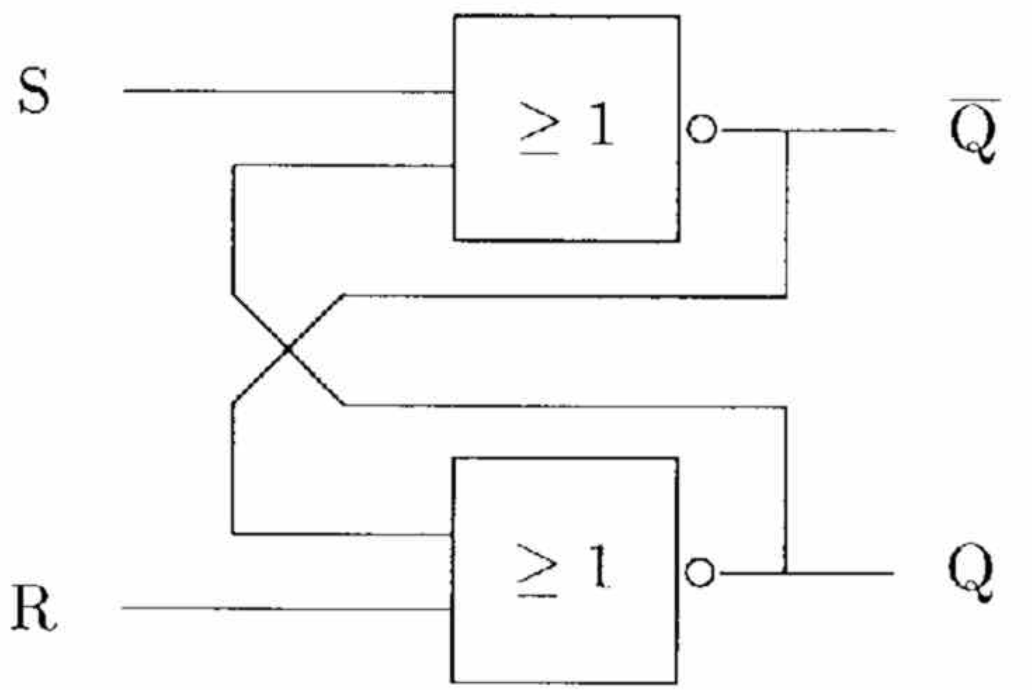
\includegraphics[height=2.5cm, keepaspectratio]{images/rsflipflop.png}}%
    \caption{RS-Flipflop}%
    \label{fig:rsflipflop}
  \endminipage\hspace{1cm}   
%
  \minipage{0.4\textwidth}
    \fbox{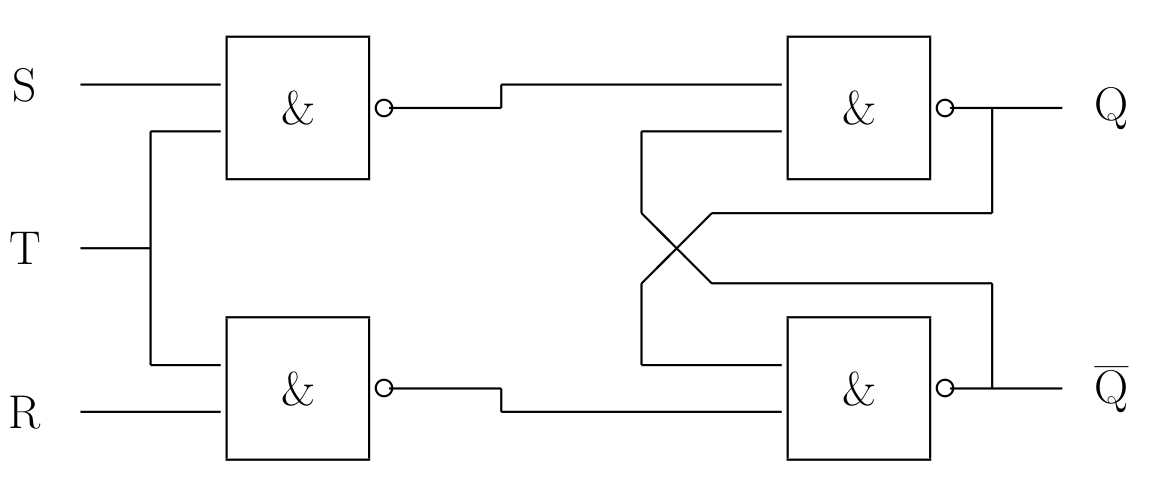
\includegraphics[height=2.5cm, keepaspectratio]{images/rsflipfloptakt.png}}%
    \caption{getaktetes RS-Flipflop}%
    \label{fig:rsflipfloptakt}
  \endminipage
\end{figure}

Referencing: Figure \ref{fig:rsflipflop}, Figure \ref{fig:rsflipfloptakt}).



Fusce suscipit mauris a justo dignissim, sit amet cursus lacus blandit. Aenean quis interdum ipsum. Integer scelerisque lacus eu lacinia vulputate. Nunc vitae pulvinar nisi. In eget pulvinar ante. Donec ultrices nec erat non porta. Ut feugiat ligula et finibus rutrum. Cras varius congue sapien, id pulvinar mi fringilla et.
%
\piccaption{Darstellung des Zahlenbereichs des Zweierkomplements mit acht Stellen\label{fig:tabelle_zweierkomplement}}
\parpic[r]{%
	\fbox{
		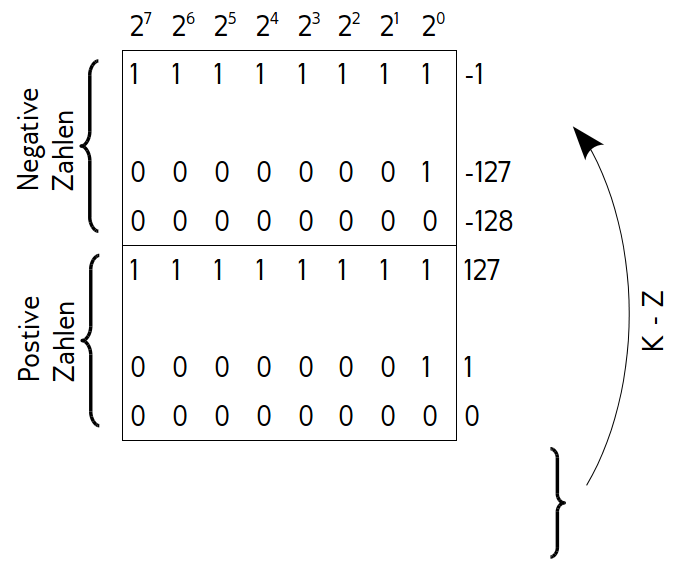
\includegraphics[width = 5.5cm, keepaspectratio]{images/tabelle_zweierkomplement.png}
	}
}
%
Lorem ipsum dolor sit amet, consectetur adipiscing elit. Vivamus sodales cursus finibus. Vestibulum ante ipsum primis in faucibus orci luctus et ultrices posuere cubilia Curae; Vestibulum sagittis faucibus felis ut efficitur. Donec vel pretium enim. Nulla ut urna facilisis, fringilla mauris id, aliquam arcu. Pellentesque tincidunt dapibus aliquet. Aliquam iaculis, risus molestie efficitur ultrices, nibh sapien mattis urna, non iaculis dolor mauris a nisl. Nam imperdiet, dui sit amet vestibulum rutrum, justo massa luctus magna, a aliquet risus ligula ultricies erat. Ut fermentum volutpat arcu ac auctor. In condimentum vehicula placerat. Nunc placerat eros id eros sagittis, et auctor lacus blandit. Donec blandit est nec sapien faucibus dapibus.

\subsection{Tables}
\begin{center}
	\begin{tabular}[c]{c | c | c || c| c | c || c | c || c | c | c || c| c| c}
		\multicolumn{3}{c||}{Konjunktion}	&	\multicolumn{3}{c||}{Disjunktion} & \multicolumn{2}{c||}{Negation} & \multicolumn{3}{c||}{NAND} & \multicolumn{3}{c}{NOR}\\
		\multicolumn{3}{c||}{UND}	&	\multicolumn{3}{c||}{ODER} & \multicolumn{2}{c||}{} & \multicolumn{3}{c||}{} & \multicolumn{3}{c}{}\\
		\hline
		$a$ & $b$ & $a$ $\wedge$ $b$ & $a$ & $b$ & $a$ $\vee$ $b$ & $a$ & $\bar{a}$ & $a$ & $b$ & $\overline{a \wedge b}$ & $a$ & $b$ & $\overline{a \vee b}$\\
		\hline
		0 & 0 & 0 & 0 & 0 & 0 & 0 & 1 & 0 & 0 & 1 & 0 & 0 & 1\\
		0 & 1 & 0 & 0 & 1 & 1 & 1 & 0 & 0 & 1 & 1 & 0 & 1 & 0\\
		1 & 0 & 0 & 1 & 0 & 1 & & & 1 & 0 & 1 & 1 & 0 & 0\\
		1 & 1 & 1 & 1 & 1 & 1 & & & 1 & 1 & 0 & 1 & 1 & 0\\
		\hline
	\end{tabular}
\end{center}

\end{appendices}


\end{document}